% Provenance (never printed): see sources/outline_sources.md (Year 2: monsoons; El Niño--Southern
% Oscillation; the North Atlantic Oscillation; ocean--atmosphere coupling). Definitions after the
% IPCC AR6 glossary, the NOAA CPC ENSO FAQ and NAO pages, the NWS glossary and the IMD monsoon
% FAQ; indices from the CPC data files (data/derived/bachelor-2-{oni,oni-table,roni,nino34,nao});
% figures from figdata/bachelor-2/climvar.py; values of the examples, exercises and problem
% computed in the Book 4 scratch calculator calc/ch23.py.
\chapter{जलवायु परिवर्तिता}\label{ch:b2:climate-variability}

सितंबर 2026 में मध्य भूमध्यरेखीय प्रशांत में समुद्र-सतह का औसत तापमान \qty{29.27}{\celsius} रहा,
जहाँ सितंबर का सामान्य मान \qty{26.71}{\celsius} है; और पूर्व में महासागर के कुछ भाग सामान्य से
\qty{4}{\celsius} से अधिक गर्म थे, और पूर्वानुमानकर्ताओं ने पाँच में चार से अधिक
संभावना बताई कि वर्ष के अंत तक यह घटना 1950 के बाद के हर एल~नीनो से आगे निकल जाएगी। पहले की
रिकॉर्ड घटनाओं ने, 1982, 1997 और 2015 में, प्रवालों को विरंजित करके मारा, उष्णकटिबंधीय वनों में आग लगाई
और लू लाईं; जब ऐसा गर्म जल टिका रहता है तो पेरू की एंकोवी मछली की पकड़ तेज़ी से गिरती है।
उष्णकटिबंधीय प्रशांत का महासागर और वायुमंडल, जैसा वे हर कुछ वर्षों में करते हैं, झूल गए थे, और यह
झूला प्रशांत से बहुत दूर तक पहुँचा। यह अध्याय जलवायु के ऐसे झूलों का वर्णन करता है: \omterm{def:b2:climate-variability:monsoon}{मानसून}, एल~नीनो
और ला~नीना, \omterm{def:b2:climate-variability:nao}{उत्तर अटलांटिक दोलन}, और वह जो महासागर को उनकी
स्मृति बनाता है।
% ledger: data:b4-nino34, cpc:edd-2026-10, thirumalai24:bjerknes, cheung26:peru

\begin{recall}
\textbf{स्कूल की पुस्तकों से}: मौसम और जलवायु; तापमान विसंगति; मिश्रित परत,
ताप-प्रवणता परत और उत्स्रवण; जलवायु प्रतिपुष्टि। \textbf{पुस्तक 3 (स्नातक वर्ष 1) से}: हैडली
कोष्ठ, व्यापारिक पवनें, अंतरोष्ण अभिसरण क्षेत्र और उसका ऋतुवार खिसकाव, वॉकर
परिसंचरण, तटीय उत्स्रवण। \textbf{\cref{ch:b2:weather-systems} से}: जेट धारा,
\omterm{def:b2:weather-systems:rossby}{रॉस्बी तरंगें}, \omterm{def:b2:weather-systems:cyclones}{बहिरुष्णकटिबंधीय चक्रवात} और अवरोधन। \textbf{भौतिकी की पुस्तकों से}: ऊष्मा धारिता
और ऊष्मागतिकी का पहला नियम।
\end{recall}

\section{परिवर्तिता और उसके माप}\label{sec:b2:climate-variability:measures}

मौसम दिन-प्रतिदिन बदलता है; जलवायु, यानी मौसम का सांख्यिकीय स्वरूप, भी बदलती है, एक ऋतु
या एक वर्ष से अगले तक, तब भी जब जलवायु तंत्र के बाहर कुछ नहीं बदलता। उस परिवर्तिता का
कुछ भाग रव है, पर उसका अधिकांश कुछ ऐसे प्रतिरूपों में संगठित है जो बार-बार लौटते हैं, अपने
भूगोल और अपने समय-पैमानों के साथ।

\begin{definition}[जलवायु परिवर्तिता की विधा; जलवायु सूचकांक; जलवायु-माध्य]\label{def:b2:climate-variability:modes}
\emph{जलवायु परिवर्तिता की विधा}\index{जलवायु परिवर्तिता की विधा} जलवायु तंत्र की प्राकृतिक
परिवर्तिता का एक बार-बार लौटने वाला प्रतिरूप है, जिसका अपना स्थानिक प्रतिरूप, ऋतुनिष्ठता और समय-पैमाने
होते हैं, और जो वायुमंडल की गतिकी से या महासागर और वायुमंडल के युग्मन से उत्पन्न होता है।
\emph{जलवायु सूचकांक}\index{जलवायु सूचकांक} जलवायु चरों से बनी एक काल-श्रेणी है
जो ऐसे प्रतिरूप की अवस्था का सार देती है, उदाहरण के लिए आइसलैंड और एज़ोर्स के बीच समुद्र-तल
दाब का अंतर। किसी चर का \emph{जलवायु-माध्य}\index{जलवायु-माध्य}
एक संदर्भ अवधि पर उसका माध्य है, जो हर कैलेंडर माह या ऋतु के लिए परिकलित होता है; मानक
संदर्भ अवधि 30 वर्ष लंबी है, इस समय 1991--2020।
\end{definition}
% ledger: ipccgl:modes, ipccgl:index, wmo:normal-30yr

अनेक विधाएँ जलवायु तंत्र के भीतर की प्रक्रियाओं से चलती हैं: वे उसकी
आंतरिक परिवर्तिता का अंग हैं। क्योंकि वे अपने समय-पैमानों के साथ लौटती हैं, वे मौसम पूर्वानुमानों की
पहुँच से आगे, सप्ताहों से दशकों तक, पूर्वानुमेयता का स्रोत हैं। सूचकांक उन्हें मापने योग्य बनाते हैं।
सूचकांक विसंगतियों से परिकलित किया जाता है, जैसा स्कूल की पुस्तकों में, और
चिकना किया जाता है।
% ledger: ipccgl:modes

\begin{method}[प्रेक्षणों से सूचकांक तक]\label{met:b2:climate-variability:index}
\begin{enumerate}
  \item \omterm{def:b2:climate-variability:modes}{जलवायु-माध्य} परिकलित कीजिए: संदर्भ अवधि पर हर कैलेंडर माह के लिए चर का
        माध्य।
  \item उसे घटाइए: हर माह की विसंगति उसका मान घटा उस माह का \omterm{def:b2:climate-variability:modes}{जलवायु-माध्य} है।
        ऋतु-चक्र लुप्त हो जाता है; जो बचता है वह परिवर्तिता है।
  \item विसंगतियों को एक चल माध्य से चिकना कीजिए, यानी हर माह पर केंद्रित $n$ क्रमागत मानों का माध्य,
        ताकि रुचि के प्रतिरूप से छोटे उतार-चढ़ाव हट जाएँ।
  \item यदि सूचकांक की तुलना दूसरों से करनी है, तो उसे उसके मानक विचलन से भाग दीजिए: तब सूचकांक
        मानकीकृत होता है, मानक विचलनों की इकाई में।
\end{enumerate}
\end{method}

\begin{example}[एक विसंगति]\label{ex:b2:climate-variability:anomaly}
\ang{5} उ और \ang{5} द, \ang{170} प और \ang{120} प के बीच मध्य भूमध्यरेखीय प्रशांत का
माध्य समुद्र-सतह तापमान सितंबर 2026 में \qty{29.27}{\celsius} था। उसका सितंबर का
\omterm{def:b2:climate-variability:modes}{जलवायु-माध्य} \qty{26.71}{\celsius} है, अतः विसंगति $29.27 - 26.71 = \qty{2.56}{\celsius}$ थी।
सितंबर 1997 में वही महासागर \qty{28.79}{\celsius} पर था, जबकि \omterm{def:b2:climate-variability:modes}{जलवायु-माध्य} \qty{26.73}{\celsius} था, यानी
\qty{2.06}{\celsius} की विसंगति। दोनों \omterm{def:b2:climate-variability:modes}{जलवायु-माध्य} थोड़े भिन्न हैं क्योंकि संदर्भ
अवधि हर पाँच वर्ष में खिसकाई जाती है: महासागर स्वयं गर्म हुआ है।
% ledger: data:b4-nino34, cpc:oni-def
\end{example}

\section{मानसून}\label{sec:b2:climate-variability:monsoons}

\begin{definition}[मानसून]\label{def:b2:climate-variability:monsoon}
\emph{मानसून}\index{मानसून} एक तापीय रूप से चालित पवन है, जो किसी भू-भाग और निकटवर्ती महासागर के
भिन्न तापन से उत्पन्न होती है और ऋतुओं के साथ अपनी दिशा उलट देती है, साथ में उससे आने वाला
वर्षा का ऋतुवार उलटाव भी।
\end{definition}
% ledger: nws4:monsoon, ipccgl:monsoon

भूमि पर ग्रीष्म के सूर्य की ऊष्मा सतह के निकट एक पतली परत में रहती है, जबकि समुद्र उसी ऊष्मा को
दसियों मीटर गहरी अपनी मिश्रित परत में नीचे तक मिला देता है, और बहुत कम गर्म होता है। भूमि के ऊपर की
वायु अधिक गर्म होती है, सतह पर उसका दाब गिरता है, और समुद्र से नम वायु भीतर बहती है, उठती है, ठंडी होती है और
बरसती है; ऊपर वायु समुद्र की ओर लौटती है। शीत ऋतु में भूमि ठंडी सतह होती है और परिसंचरण
उलट जाता है। साथ मिलाकर, ग्रह के \omterm{def:b2:climate-variability:monsoon}{मानसून} एक अकेला वैश्विक प्रतिरूप बनाते हैं जो उष्णकटिबंधीय और
उपोष्णकटिबंधीय वर्षा के वार्षिक चक्र पर हावी है; उसका क्षेत्र उन प्रदेशों के रूप में परिभाषित है जहाँ स्थानीय
ग्रीष्म की माध्य वर्षा शीत ऋतु की वर्षा से प्रतिदिन \qty{2.5}{mm} से अधिक होती है।
% ledger: nws4:monsoon, ipccgl:monsoon

\begin{omfigure}
\centering
\begin{tikzpicture}[font=\scriptsize, >=Stealth]
\foreach \col/\title in {0/{क\enspace ग्रीष्म}, 7.2/{ख\enspace शीत ऋतु}} {
  \begin{scope}[shift={(\col,0)}]
  \node[anchor=south west] at (0,3.0) {\textbf{\title}};
  \fill[ocBlue!18] (0,0) rectangle (3,0.35);
  \fill[brown!35] (3,0) -- (6.4,0) -- (6.4,0.5) -- (3,0.35) -- cycle;
  \node at (1.5,0.17) {समुद्र};
  \node at (4.7,0.2) {भूमि};
  \end{scope}
}
% summer: low over the land, inflow from the sea, rising air and rain
\node[font=\small\bfseries, ocBlue] at (0.45,0.62) {H};
\node[font=\small\bfseries, ocRed] at (4.8,0.78) {L};
\node[ocRed, anchor=west] at (5.35,0.78) {गर्म};
\draw[->, thick] (1.0,0.98) -- (4.2,1.02);
\node at (2.4,0.66) {समुद्र से नम वायु};
\draw[->, thick] (4.8,1.15) -- (4.8,2.55);
\draw[->, thick] (4.45,2.8) -- (1.75,2.8);
\draw[->, thick] (1.4,2.6) -- (1.4,1.25);
\fill[black!15, draw=black!40] (4.0,1.9) .. controls (4.0,2.55) and (5.6,2.55) .. (5.6,1.9) -- cycle;
\foreach \x in {4.25,4.5,5.1,5.35} {\draw[ocBlue, dashed] (\x,1.85) -- (\x-0.1,1.2);}
\node[anchor=west] at (5.65,2.1) {वर्षा};
% winter: high over the land, dry outflow to the sea
\begin{scope}[shift={(7.2,0)}]
\node[font=\small\bfseries, ocRed] at (0.45,0.62) {L};
\node[font=\small\bfseries, ocBlue] at (4.8,0.78) {H};
\node[ocBlue, anchor=west] at (5.35,0.78) {ठंडी};
\draw[->, thick] (4.2,1.02) -- (1.0,0.98);
\node at (2.4,0.66) {भूमि से शुष्क वायु};
\draw[->, thick] (1.4,1.25) -- (1.4,2.6);
\draw[->, thick] (1.75,2.8) -- (4.45,2.8);
\draw[->, thick] (4.8,2.55) -- (4.8,1.15);
\end{scope}
\end{tikzpicture}
\par\smallskip{\small भूमि--समुद्र परिसंचरण के रूप में \omterm{def:b2:climate-variability:monsoon}{मानसून} (योजनामूलक काट, पैमाने के बिना): ग्रीष्म में
भूमि अधिक गर्म सतह होती है, जहाँ भूमि पर निम्न दाब, समुद्र से नम वायु का अंतर्वाह,
उठती वायु और वर्षा होती है; शीत ऋतु में परिसंचरण उलट जाता है और स्थल-पवन शुष्क होती है।}
\end{omfigure}
% ledger: nws4:monsoon, imd:heat-low

दक्षिण और दक्षिण-पूर्व एशिया का \omterm{def:b2:climate-variability:monsoon}{मानसून} मई के अंत या जून के आरंभ में शुरू होता है, उत्तर-पूर्व की ओर
बढ़ता है और सितंबर के अंत या अक्तूबर के आरंभ में समाप्त होता है। उससे पहले
अरब सागर के आसपास की भूमियाँ गर्म होती हैं: जून में भारत के शुष्क उत्तर-पश्चिम, पाकिस्तान और मध्य-पूर्व के ऊपर सतह
वायु में लगभग \qty{160}{W/m^2} ऊष्मा भेजती है, और वहाँ एक उथला ऊष्मीय निम्न दाब बनता है,
जो केवल लगभग \qty{1.5}{km} तक पहुँचता है, थोड़ी वर्षा के साथ; दुर्बल ऊष्मीय निम्न दाब, जैसा सूखे के वर्ष
1987 में, महासागर की नम वायु पर दुर्बल खिंचाव का संकेत है। उससे निम्न दाब की एक लंबी द्रोणिका, \omterm{def:b2:climate-variability:monsoon}{मानसून}
द्रोणिका, बंगाल की खाड़ी के शीर्ष तक जाती है; उसके उत्तर--दक्षिण दोलन ऋतु के सक्रिय
दौर और विराम लाते हैं। पूरे भारत पर जून से सितंबर की वर्षा का औसत
\qty{88}{cm} है, \qty{9}{cm} के मानक विचलन के साथ, लगभग \qty{10}{\percent}: जो ऋतु दीर्घावधि औसत के
\qty{10}{\percent} के भीतर हो उसे सामान्य कहते हैं। केरल तट पर, जहाँ
राष्ट्रीय मौसम सेवा चौदह केंद्रों की वर्षा, पवनों और उपग्रह से मापे गए बहिर्गामी
अवरक्त विकिरण से \omterm{def:b2:climate-variability:monsoon}{मानसून} के आगमन की घोषणा करती है, औसत वर्षा जून में
\qty{556}{mm} और जुलाई में \qty{659}{mm} है।
% ledger: ipccgl:monsoon, imd:heat-low, imd:lpa, imd:onset

पश्चिम अफ़्रीकी \omterm{def:b2:climate-variability:monsoon}{मानसून} गिनी की खाड़ी से नम दक्षिण-पश्चिमी पवनें लाता है, जो मई से सितंबर तक
उत्तर की ओर बढ़ती हैं; उसकी वर्षा अगस्त के अंत और सितंबर में \ang{12} उ के निकट शिखर पर पहुँचती है और
अक्तूबर से पीछे हटती है।
% ledger: ipccgl:monsoon

\omterm{def:b2:climate-variability:monsoon}{मानसून} अपने समय में नियमित है, अपनी मात्रा में अनियमित, और उष्णकटिबंधीय प्रशांत के वर्ष-दर-वर्ष के झूले
उसके कारणों में से हैं। एल~नीनो वर्ष भारत को वर्षा की कमी में छोड़ने की प्रवृत्ति रखते हैं:
1904, 1972 और 1987 के सूखे एल~नीनो के साथ आए। यह संबंध निश्चित नहीं है: 1997 में एक प्रबल
एल~नीनो हिंद महासागर द्विध्रुव की धनात्मक प्रावस्था के साथ पड़ा, एक विधा जो आगे मिलेगी, और भारत में
लगभग सामान्य \omterm{def:b2:climate-variability:monsoon}{मानसून} रहा।
% ledger: narang24:enso-monsoon, ipccgl:other-modes

\section{एल नीनो और दक्षिणी दोलन}\label{sec:b2:climate-variability:enso}

पुस्तक 3 (स्नातक वर्ष 1) ने वॉकर परिसंचरण का वर्णन किया था: गर्म पश्चिमी प्रशांत के ऊपर उठती वायु,
ऊपर पूर्व की ओर बहती, ठंडे पूर्वी प्रशांत के ऊपर नीचे उतरती और व्यापारिक पवनों के साथ
पश्चिम की ओर लौटती। नीचे महासागर में व्यापारिक पवनें गर्म जल को पश्चिम में जमा करती हैं, जहाँ ताप-प्रवणता परत
गहरी है, और पूर्व में भूमध्यरेखा के अनुदिश ठंडा जल ऊपर खींचती हैं, जहाँ वह उथली है। यह अवस्था
स्थिर नहीं है।

\begin{definition}[एल नीनो--दक्षिणी दोलन; एल नीनो; ला नीना; दक्षिणी दोलन]\label{def:b2:climate-variability:enso}
\emph{एल नीनो--दक्षिणी दोलन}\index{एल नीनो--दक्षिणी दोलन} (ENSO) उष्णकटिबंधीय प्रशांत की
युग्मित महासागर--वायुमंडल विधा है: भूमध्यरेखीय प्रशांत के अनुदिश समुद्र-सतह तापमान, संवहनी वर्षा, सतही दाब
और परिसंचरण के सुसंगत वर्ष-दर-वर्ष परिवर्तन,
दो से लगभग सात वर्षों के वरीय समय-पैमानों के साथ। \emph{एल
नीनो}\index{एल नीनो} उसकी उष्ण प्रावस्था है, मध्य और पूर्व-मध्य भूमध्यरेखीय प्रशांत की
समुद्र-सतह का गर्म होना; \emph{ला नीना}\index{ला नीना} उसकी शीत प्रावस्था है, उसी क्षेत्र का
ठंडा होना। \emph{दक्षिणी दोलन}\index{दक्षिणी दोलन} उसका वायुमंडलीय अंश है,
पश्चिमी और पूर्वी उष्णकटिबंधीय प्रशांत के बीच सतही दाब का एक झूला: एल~नीनो के दौरान
इंडोनेशिया और पश्चिमी प्रशांत के ऊपर दाब औसत से अधिक और पूर्वी प्रशांत के ऊपर कम होता है,
और ला~नीना के दौरान इसका उलटा।
\end{definition}
% ledger: cpc:enso-faq, cpc:enso-faq-so, ipccgl:enso

एल~नीनो के दौरान भूमध्यरेखा के अनुदिश पूर्वी व्यापारिक पवनें दुर्बल होती हैं, और पश्चिम में
निचले स्तर की पवनें पश्चिम से भी बह सकती हैं; पश्चिम का गर्म जल पूर्व की ओर फैलता है, और गहरा
संवहन और उसकी वर्षा उसके पीछे चलते हैं, जिससे इंडोनेशिया और उत्तरी ऑस्ट्रेलिया अधिक शुष्क रह जाते हैं।
पूर्व-मध्य प्रशांत की समुद्र-सतह सामान्यतः औसत से \qtyrange{1.5}{2.5}{\celsius} अधिक गर्म होती है, और
वहाँ ताप-प्रवणता परत \qtyrange{150}{175}{m} पर, सामान्य से गहरी, होती है। ला~नीना के दौरान व्यापारिक
पवनें पूरी द्रोणी में प्रबल होती हैं, समुद्र-सतह औसत से \qtyrange{1}{2}{\celsius} ठंडी होती है, और
पूर्व में ताप-प्रवणता परत \qtyrange{50}{100}{m} तक ऊपर उठ आती है। वॉकर परिसंचरण
एल~नीनो के दौरान दुर्बल और ला~नीना के दौरान प्रबल होता है। घटनाएँ सामान्यतः हर तीन से
पाँच वर्ष में लौटती हैं, ऐसे अंतरालों पर जो दो से सात वर्ष तक रहे हैं; एक एल~नीनो सामान्यतः नौ से
बारह महीने चलता है, एक ला~नीना एक से तीन वर्ष। दोनों मार्च और जून के बीच विकसित होने,
दिसंबर और अप्रैल के बीच शिखर पर पहुँचने और मई और जुलाई के बीच दुर्बल होने की प्रवृत्ति रखते हैं; उनके
प्रभाव दिसंबर से अप्रैल तक सबसे प्रबल होते हैं, जब भूमध्यरेखीय समुद्र-सतह सबसे गर्म होती है।
% ledger: cpc:enso-faq-features, cpc:enso-faq-timing

\begin{omfigure}
\centering
\begin{tikzpicture}[font=\scriptsize, >=Stealth, x=1cm, y=0.8cm]
\foreach \row/\title/\tw/\te/\rx/\cwidth in {
    0/{क\enspace उदासीन}/1.15/0.35/1.6/1.0,
    -4.6/{ख\enspace एल नीनो}/0.95/0.85/5.6/1.4,
    -9.2/{ग\enspace ला नीना}/1.3/0.18/1.0/0.8} {
  \begin{scope}[shift={(0,\row)}]
  \node[anchor=south west] at (0,2.55) {\textbf{\title}};
  % ocean: warm layer above the thermocline
  \fill[ocBlue!20] (0,-1.5) rectangle (11,0);
  \fill[omWarm!25] (0,0) -- (0,-\tw) .. controls (4,-\tw) and (7,-\te) .. (11,-\te) -- (11,0) -- cycle;
  \draw[thick, ocBlue!70!black] (0,-\tw) .. controls (4,-\tw) and (7,-\te) .. (11,-\te);
  \draw (0,0) -- (11,0);
  % convection and Walker cell
  \fill[black!15, draw=black!40] ({\rx-\cwidth/2},0.5) .. controls ({\rx-\cwidth/2},2.1) and ({\rx+\cwidth/2},2.1) .. ({\rx+\cwidth/2},0.5) -- cycle;
  \draw[->, thick] (\rx,0.55) -- (\rx,2.15);
  \draw[->, thick] ({\rx+0.4},2.3) -- (9.6,2.3);
  \draw[->, thick] (10.0,2.1) -- (10.0,0.5);
  \draw[->, thick] (9.6,0.3) -- ({\rx+0.7},0.3);
  \end{scope}
}
\node[anchor=west] at (2.3,1.4) {उठती वायु, वर्षा};
\node[anchor=east] at (9.9,1.4) {उतरती वायु};
\node at (6.0,0.55) {व्यापारिक पवनें};
\node[anchor=west, ocBlue!70!black] at (7.6,-0.95) {ताप-प्रवणता परत};
\node[anchor=east] at (4.8,-4.6+1.4) {वर्षा पूर्व की ओर खिसकती है};
\node at (8.2,-4.6+0.55) {दुर्बल व्यापारिक पवनें};
\node at (6.0,-9.2+0.55) {प्रबल व्यापारिक पवनें};
\node[ocBlue!70!black, align=center] at (9.6,-9.2-0.8) {सतह के निकट\\ठंडा जल};
\node[anchor=north west] at (0,-9.2-1.55) {पश्चिम (इंडोनेशिया)};
\node[anchor=north east] at (11,-9.2-1.55) {पूर्व (दक्षिण अमेरिका)};
\end{tikzpicture}
\par\smallskip{\small ENSO की तीन प्रावस्थाओं में भूमध्यरेखा के अनुदिश भूमध्यरेखीय प्रशांत
(योजनामूलक, पैमाने के बिना): ऊपर वॉकर परिसंचरण, नीचे गर्म ऊपरी परत और
ताप-प्रवणता परत। एल~नीनो के दौरान व्यापारिक पवनें दुर्बल होती हैं, गर्म जल और वर्षा पूर्व की ओर फैलते हैं
और पूर्व में ताप-प्रवणता परत \qtyrange{150}{175}{m} तक गहरी हो जाती है; ला~नीना के दौरान व्यापारिक पवनें
प्रबल होती हैं और पूर्व में ताप-प्रवणता परत \qtyrange{50}{100}{m} तक ऊपर उठती है।}
\end{omfigure}
% ledger: cpc:enso-faq-features, climategov:walker

ये नाम भिन्न शताब्दियों और भिन्न विज्ञानों से आए हैं। दक्षिण अमेरिका के तट के मछुआरों ने
क्रिसमस के आसपास अपने तटीय जल का गर्म होना देखा जो मत्स्य-ग्रहण को बाधित करता था, और उसे एल~नीनो,
यानी बालक, कहा। सर गिल्बर्ट वॉकर ने वायुमंडल में \omterm{def:b2:climate-variability:enso}{दक्षिणी दोलन} की खोज की, उसे महासागर से जोड़े बिना।
1960 के दशक के अंत में ही जैकब ब्येर्कनेस और अन्य ने देखा कि
दोनों एक ही परिघटना हैं। ला~नीना और उदासीन शब्द 1980 के दशक में प्रमुख हुए।
% ledger: climategov:enso-history, ipccgl:enso

\begin{history}[मछुआरों का बालक]
\begin{minipage}[t]{0.54\linewidth}\vspace{0pt}
पेरू के शुष्क तट के पास, जो ठंडा जल पवनें तट के अनुदिश ऊपर खींचती हैं वह पोषक तत्त्वों से भरपूर है और
एक उत्पादक मत्स्य-क्षेत्र को पोषण देता है। उसके मछुआरे एक ऐसे गर्म होने को जानते थे जो क्रिसमस के आसपास
आता था, जब मछलियाँ दुर्लभ हो जाती थीं, और उन्होंने उसे उस ऋतु के शिशु का नाम दिया। पेरू की
एंकोवी पकड़ अब भी ENSO का अनुसरण करती है: एक हाल के विश्लेषण में, लंबे समय तक बनी उच्च तापमान
विसंगतियों ने अत्यंत कम पकड़ को नौ गुना से अधिक संभाव्य बना दिया, पकड़ में लगभग \qty{60}{\percent} की
माध्यिका गिरावट के साथ; 1997--98 का प्रबल एल~नीनो अभिलेख में अलग दिखता है।
\end{minipage}\hfill
\begin{minipage}[t]{0.42\linewidth}\vspace{0pt}
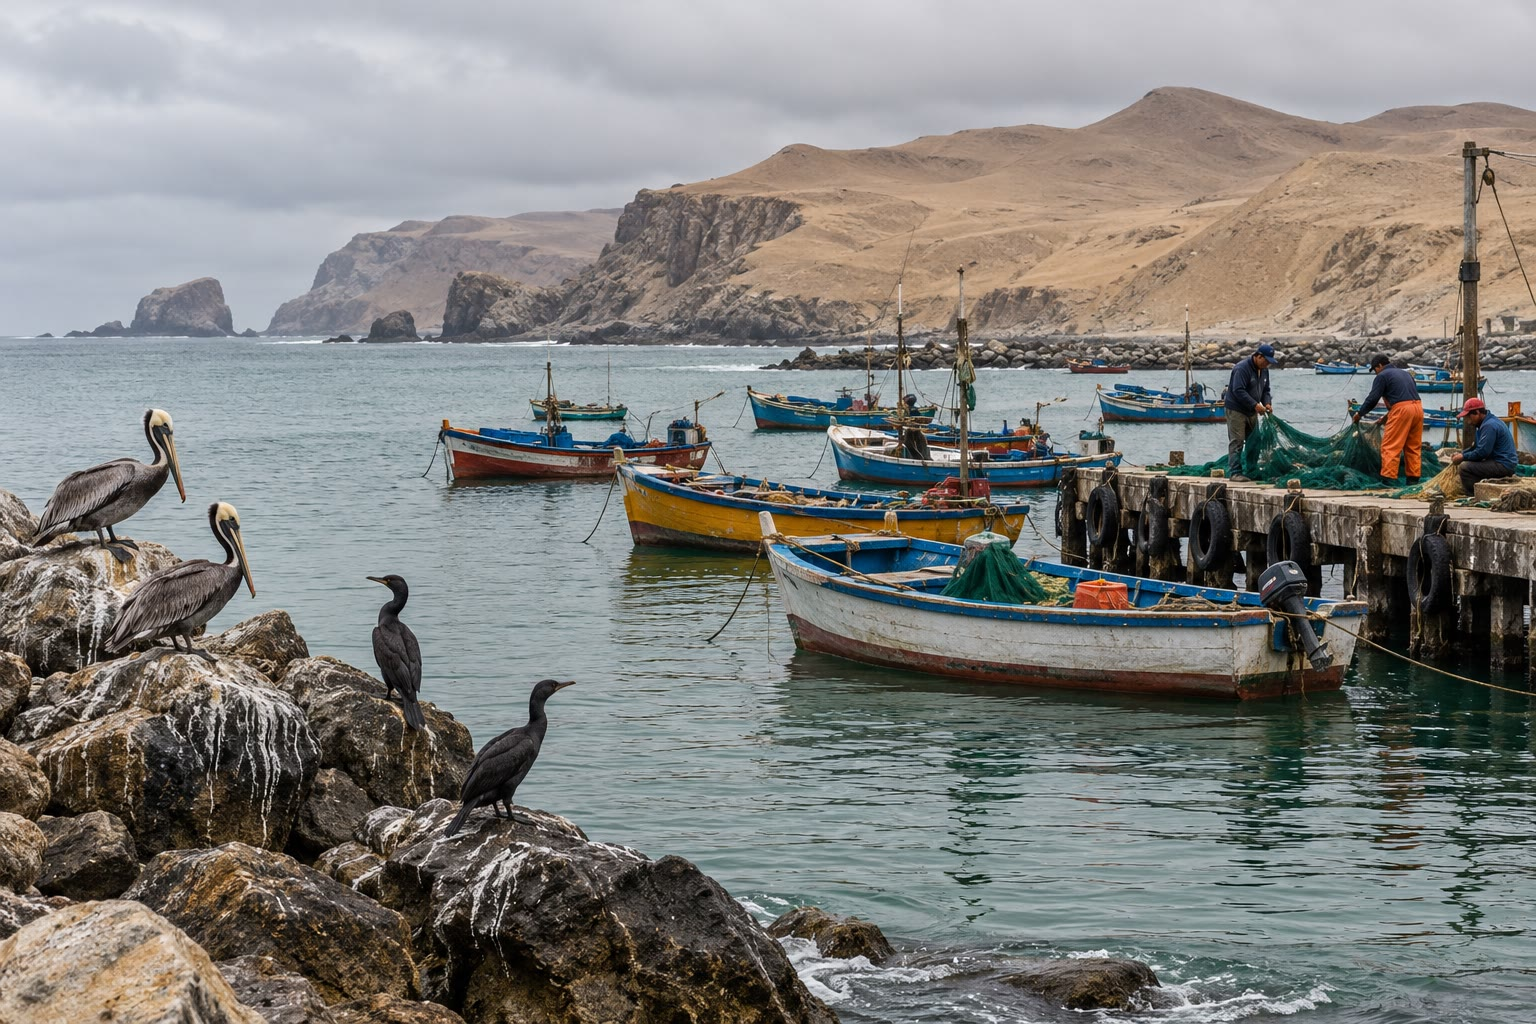
\includegraphics[width=\linewidth]{images/book4/ai/b2-fishing-harbour.jpg}

{\scriptsize ठंडे उत्स्रवित जल वाले मरुस्थलीय तट के एक बंदरगाह में मछली पकड़ने वाली नावें
(AI से बनाया गया चित्रण)।}
\end{minipage}
% ledger: climategov:enso-history, cheung26:peru, stewart:upwelling
\end{history}

तंत्र झूलता ही क्यों है? क्योंकि भूमध्यरेखीय प्रशांत के महासागर और वायुमंडल
एक-दूसरे की विसंगतियों को सुदृढ़ करते हैं।

\begin{definition}[ब्येर्कनेस प्रतिपुष्टि]\label{def:b2:climate-variability:bjerknes}
\emph{ब्येर्कनेस प्रतिपुष्टि}\index{ब्येर्कनेस प्रतिपुष्टि} भूमध्यरेखीय प्रशांत के
समुद्र-सतह तापमान, पवनों और महासागरीय धाराओं के बीच की धनात्मक प्रतिपुष्टि है: पूर्व का गर्म होना
तापमान और दाब के पूर्व--पश्चिम अंतर को, और इसलिए व्यापारिक पवनों को, दुर्बल करता है;
दुर्बल व्यापारिक पवनें पश्चिम के गर्म जल को पूर्व की ओर फैलने देती हैं और पूर्व में कम ठंडा जल
ऊपर लाती हैं, जो पूर्व को और गर्म करता है। यही चक्र किसी ठंडे होने को भी बढ़ाता है।
\end{definition}
% ledger: thirumalai24:bjerknes, cpc:enso-faq-timing

\begin{omfigure}
\centering
\begin{tikzpicture}[font=\small, >=Stealth, box/.style={draw, rounded corners=2pt, fill=omDef!8,
  align=center, text width=4.3cm, minimum height=1.05cm, inner sep=3pt}]
\node[box] (a) at (0,2) {पूर्वी भूमध्यरेखीय प्रशांत\\सामान्य से अधिक गर्म};
\node[box] (b) at (6.2,2) {तापमान और दाब का\\छोटा पूर्व--पश्चिम अंतर};
\node[box] (c) at (6.2,0) {दुर्बल व्यापारिक पवनें};
\node[box] (d) at (0,0) {गर्म जल पूर्व की ओर फैलता है,\\कम ठंडा जल ऊपर आता है};
\draw[->, very thick, ocRed] (a) -- (b);
\draw[->, very thick, ocRed] (b) -- (c);
\draw[->, very thick, ocRed] (c) -- (d);
\draw[->, very thick, ocRed] (d) -- (a);
\node[ocRed, font=\bfseries] at (3.1,1) {$+$};
\end{tikzpicture}
\par\smallskip{\small \omterm{def:b2:climate-variability:bjerknes}{ब्येर्कनेस प्रतिपुष्टि}, गर्म होने के लिए खींची गई; हर तीर उलट देने पर
यही चक्र ठंडे होने को गहरा करता है। इस प्रकार का धनात्मक चक्र छोटे विक्षोभ को बढ़ाता है।}
\end{omfigure}
% ledger: thirumalai24:bjerknes

धनात्मक प्रतिपुष्टि यह समझाती है कि विसंगति कैसे बढ़ती है, यह नहीं कि वह कैसे शुरू या समाप्त होती है। एक वर्तमान
व्याख्या में एल~नीनो तब शुरू होता है जब व्यापारिक पवनों के यादृच्छिक उतार-चढ़ाव उन भूमध्यरेखीय धाराओं को दुर्बल कर देते हैं जो
गर्म जल को पश्चिम में रोके रखती हैं; उष्ण कुंड पूर्व की ओर फैलता है, संवहन उसके पीछे चलता है,
\omterm{def:b2:climate-variability:bjerknes}{ब्येर्कनेस प्रतिपुष्टि} नियंत्रण ले लेती है और घटना बढ़ती है। उसी व्याख्या में ला~नीना घटनाएँ
किसी पूर्ववर्ती एल~नीनो से शुरू होती हैं। तंत्र को दोलित कराने वाले सबसे सरल मॉडल, जिनमें पुनर्भरण
दोलित्र भी है, दो राशियों को युग्मित करते हैं: मध्य प्रशांत की समुद्र-सतह तापमान विसंगति
और भूमध्यरेखा के अनुदिश संचित गर्म ऊपरी-महासागर जल का आयतन। तापमान
विसंगति अपने द्वारा चलाई गई पवनों के माध्यम से उस भंडार को खाली करती या फिर भरती है, और भंडार,
ताप-प्रवणता परत की गहराई के माध्यम से, अगली प्रावस्था तैयार करता है। \Cref{exo:b2:climate-variability:10} ऐसे
समीकरण-युग्म को हल करता है।
% ledger: thirumalai24:bjerknes, stuecker25:ro

ENSO पर नज़र रखने के लिए निगरानी केंद्र सूचकांकों का उपयोग करते हैं।

\begin{definition}[नीनो-3.4 सूचकांक; महासागरीय नीनो सूचकांक]\label{def:b2:climate-variability:oni}
\emph{नीनो-3.4 सूचकांक}\index{नीनो-3.4 सूचकांक} \ang{5} उ--\ang{5} द, \ang{170} प--\ang{120} प क्षेत्र पर औसत
समुद्र-सतह तापमान की मासिक विसंगति है, वर्ष पर केंद्रित 30-वर्षीय आधार अवधि के
\omterm{def:b2:climate-variability:modes}{जलवायु-माध्य} के सापेक्ष, जो हर पाँच वर्ष में अद्यतन होती है।
\emph{महासागरीय नीनो सूचकांक}\index{महासागरीय नीनो सूचकांक} (ONI) उसका तीन-मासिक चल माध्य है। एक
एल~नीनो (ला~नीना) घटना कम से कम पाँच क्रमागत अतिव्यापी तीन-मासिक ऋतुओं का ऐसा क्रम है
जिसमें ONI \qty{+0.5}{\celsius} पर या उससे ऊपर (\qty{-0.5}{\celsius} पर या उससे नीचे) हो।
\end{definition}
% ledger: cpc:oni-def, cpc:enso-faq

ऋतुएँ अतिव्यापी हैं: DJF, JFM, FMA इत्यादि, हर एक तीन महीनों का माध्य, हर एक अगले के साथ दो
महीने साझा करती हुई। एक दूसरा सूचकांक, \omterm{def:b2:climate-variability:enso}{दक्षिणी दोलन} सूचकांक, वायुमंडल का अनुसरण करता है: वह
ताहिती और डार्विन के बीच दाब-अंतर के विचलनों से परिकलित होता है, एल~नीनो के दौरान ऋणात्मक
और ला~नीना के दौरान धनात्मक। फ़रवरी 2026 से ENSO की निगरानी का आधिकारिक सूचकांक
एक सापेक्ष ONI है, जो नीनो-3.4 विसंगति में से \ang{20} उ और \ang{20} द के बीच के पूरे
उष्णकटिबंधीय महासागर की माध्य विसंगति घटाकर परिकलित होता है, फिर ONI के आयाम पर पुनःमापित किया जाता है।
पूरे उष्णकटिबंधीय क्षेत्र के सापेक्ष मापा जाने के कारण, जब तक महासागर गर्म हो रहे हैं, वह आधार अवधि के चयन पर कम
निर्भर करता है, और उष्णकटिबंधीय प्रशांत की वर्षा से बेहतर संबंधित है। सितंबर 2026 में
नीनो-3.4 क्षेत्र की सापेक्ष विसंगति \qty{2.08}{\celsius} थी, जबकि
\cref{ex:b2:climate-variability:anomaly} की विसंगति \qty{2.56}{\celsius}: पारंपरिक विसंगति का लगभग आधा अंश
उष्णकटिबंधीय महासागरों की समग्र गर्माहट थी।
% ledger: cpc:enso-faq-so, pns:roni, data:b4-rnino34

\begin{omfigure}
\centering
% figdata/bachelor-2/climvar.py part oni
\begin{tikzpicture}
\begin{axis}[width=\linewidth, height=6.0cm, xmin=1950, xmax=2027, ymin=-2.4, ymax=3.0,
  xlabel={वर्ष}, ylabel={सूचकांक (\unit{\celsius})}, tick label style={font=\scriptsize},
  label style={font=\small}, xtick={1950,1960,...,2020}, x tick label style={/pgf/number
  format/1000 sep={}}, legend style={font=\scriptsize, at={(0.5,1.02)}, anchor=south,
  draw=none, legend columns=3, /tikz/every even column/.append style={column sep=6pt}},
  legend cell align=left]
\addplot[fill=ocRed!70, draw=none, area legend] table[x=t, y=pos]
  {figdata/out/bachelor-2-climvar-oni.dat} \closedcycle;
\addlegendentry{ONI, एल नीनो पक्ष}
\addplot[fill=ocBlue!70, draw=none, area legend] table[x=t, y=neg]
  {figdata/out/bachelor-2-climvar-oni.dat} \closedcycle;
\addlegendentry{ONI, ला नीना पक्ष}
\addplot[black, thin] table[x=t, y=roni] {figdata/out/bachelor-2-climvar-oni.dat};
\addlegendentry{सापेक्ष ONI}
\addplot[black!60, densely dashed, domain=1950:2027, samples=2] {0.5};
\addplot[black!60, densely dashed, domain=1950:2027, samples=2] {-0.5};
\end{axis}
\end{tikzpicture}
\par\smallskip{\small DJF 1950 से JAS 2026 तक \omterm{def:b2:climate-variability:oni}{महासागरीय नीनो सूचकांक} (हर
तीन-मासिक ऋतु का एक मान, उसके मध्य माह पर अंकित), और सापेक्ष ONI, जो फ़रवरी 2026 से आधिकारिक
सूचकांक है; धराशायी: देहलियाँ $\pm\qty{0.5}{\celsius}$। डेटा: NOAA Climate Prediction
Center, 23 अक्तूबर 2026 को प्राप्त।}
\end{omfigure}
% ledger: data:b4-oni, data:b4-roni

जलवायु पूर्वानुमान केंद्र की तालिका पर पाँच-ऋतु नियम से गिनने पर, ONI 1950 और 2026 की ग्रीष्म के बीच 25
एल~नीनो और 21 ला~नीना घटनाएँ दिखाता है। सबसे प्रबल एल~नीनो
शिखर 1997 के अंत में \qty{2.4}{\celsius} और 2015 के अंत में \qty{2.6}{\celsius} थे। दोनों सूचकांक
हाल के वर्षों में सबसे अधिक अलग होते हैं: जुलाई--सितंबर 2026 में ONI \qty{2.2}{\celsius} पर था और
सापेक्ष सूचकांक \qty{1.7}{\celsius} पर।
% ledger: data:b4-oni, data:b4-roni

\begin{dated}{2026}
8 अक्तूबर 2026 की अपनी चर्चा में जलवायु पूर्वानुमान केंद्र ने अपनी एल~नीनो चेतावनी बनाए रखी:
सितंबर में सापेक्ष नीनो-3.4 विसंगति \qty{+2.1}{\celsius} तक पहुँच गई थी, पूर्वी
भूमध्यरेखीय प्रशांत के कुछ भाग औसत से \qty{4}{\celsius} से अधिक ऊपर थे, पूर्व में गहराई पर जल
\qty{10}{\celsius} से अधिक ऊपर, और \omterm{def:b2:climate-variability:enso}{दक्षिणी दोलन} सूचकांक सार्थक रूप से
ऋणात्मक थे।
प्रबल से अति-प्रबल एल~नीनो के जनवरी--मार्च 2027 तक बने रहने की संभावना आँकी गई, और यह संभावना कि
सापेक्ष सूचकांक \qty{2.5}{\celsius} से आगे जाएगा, यानी 1950 के बाद की हर घटना से आगे,
अक्तूबर--दिसंबर के लिए \qty{83}{\percent} आँकी गई।
% ledger: cpc:edd-2026-10, data:b4-rnino34
\end{dated}

\section{उत्तर अटलांटिक दोलन और दूरसंबंध}\label{sec:b2:climate-variability:nao}

\begin{definition}[उत्तर अटलांटिक दोलन]\label{def:b2:climate-variability:nao}
\emph{उत्तर अटलांटिक दोलन}\index{उत्तर अटलांटिक दोलन} (NAO) उत्तर अटलांटिक के ऊपर वायुमंडलीय परिवर्तिता की
प्रमुख विधा है: आइसलैंडी निम्न और एज़ोर्स उच्च के बीच समुद्र-तल दाब का एक झूला।
उसका सूचकांक तब धनात्मक होता है जब दोनों औसत से प्रबल हों, ताकि
उनके बीच दाब-अंतर बड़ा हो, और ऋणात्मक जब दोनों दुर्बल हों।
\end{definition}
% ledger: ipccgl:other-modes, climategov:nao, cpc:nao-teledoc

NAO पिछले अध्याय की पछुआ पवनों को दिशा देता है। उसकी धनात्मक प्रावस्था में बड़ा दाब-अंतर
अधिक प्रबल अटलांटिक जेट धारा चलाता है और तूफ़ान-पथ को उत्तर की ओर खिसकाता है: उत्तरी यूरोप में
अधिक तूफ़ानी, गीली और मृदु शीत ऋतु होती है, दक्षिणी यूरोप में अधिक शुष्क, पूर्वी उत्तर अमेरिका में
ठंडी वायु के कम प्रकोप, और ग्रीनलैंड में अधिक ठंडी शीत ऋतु। ऋणात्मक प्रावस्था इन
विसंगतियों को उलट देती है। अठारहवीं शताब्दी के अंत में ही एक मिशनरी ने देखा था कि ग्रीनलैंड में मृदु शीत ऋतुएँ
डेनमार्क में कठोर शीत ऋतुओं के साथ आती थीं, और इसका उलटा भी।
% ledger: climategov:nao, cpc:nao-teledoc

NAO हर ऋतु में वायुमंडल के सबसे प्रमुख प्रतिरूपों में से एक है, और उसका एक अन्य विधा, आर्कटिक दोलन,
से प्रबल सहसंबंध है। वह दशकों के पैमाने पर भी बदलता है: ऋणात्मक प्रावस्था 1950 के दशक के मध्य से
1978--79 की शीत ऋतु तक हावी रही, और धनात्मक प्रावस्था 1979--80 से 1994--95 तक।
% ledger: cpc:nao-teledoc, climategov:nao

\begin{omfigure}
\centering
% figdata/bachelor-2/climvar.py part nao
\begin{tikzpicture}
\begin{axis}[width=\linewidth, height=5.4cm, xmin=1950, xmax=2027, ymin=-1.9, ymax=1.9,
  ytick={-1,0,1},
  xlabel={शीत ऋतु (उसकी जनवरी का वर्ष)}, ylabel={NAO सूचकांक (DJF माध्य)},
  tick label style={font=\scriptsize}, label style={font=\small}, xtick={1950,1960,...,2020},
  x tick label style={/pgf/number format/1000 sep={}}, legend style={font=\scriptsize,
  at={(0.5,1.02)}, anchor=south, draw=none, legend columns=2,
  /tikz/every even column/.append style={column sep=6pt}},
  legend cell align=left, unbounded coords=jump]
\addplot[ybar, bar width=0.6, fill=omDef!55, draw=none, area legend] table[x=year, y=nao]
  {figdata/out/bachelor-2-climvar-nao.dat};
\addlegendentry{शीत ऋतु माध्य}
\addplot[ocRed, thick] table[x=year, y=run5] {figdata/out/bachelor-2-climvar-nao.dat};
\addlegendentry{5-शीत ऋतु चल माध्य}
\end{axis}
\end{tikzpicture}
\par\smallskip{\small NOAA जलवायु पूर्वानुमान केंद्र के मासिक NAO सूचकांक का शीत ऋतु (दिसंबर--फ़रवरी) माध्य,
1951--2026, मानक विचलनों में, उसके केंद्रित पाँच-शीत ऋतु
चल माध्य के साथ। सबसे निम्न शीत ऋतु 2010 है ($-1.67$), सबसे उच्च 2015 ($+1.66$)।}
\end{omfigure}
% ledger: data:b4-nao, cpc:nao-teledoc

NAO, ENSO और अन्य विधाएँ वहाँ से बहुत दूर असर डालती हैं जहाँ उन्हें मापा जाता है।

\begin{definition}[दूरसंबंध]\label{def:b2:climate-variability:teleconnection}
\emph{दूरसंबंध}\index{दूरसंबंध} दूर-दूर स्थित, नियत स्थानों पर जलवायु चरों के बीच का एक साहचर्य है,
जो वायुमंडल या महासागर में पथों के अनुदिश भौतिक प्रक्रियाओं से जुड़ा होता है, जैसे \omterm{def:b2:weather-systems:rossby}{रॉस्बी तरंगों} की श्रृंखलाएँ,
जेट धारा और तूफ़ान-पथों के खिसकाव, या वॉकर परिसंचरण के
परिवर्तन।
\end{definition}
% ledger: ipccgl:teleconnection

एल~नीनो के दौरान उष्णकटिबंधीय वर्षा इंडोनेशिया से दक्षिण अमेरिका तक, लगभग आधी
पृथ्वी के चारों ओर, बदलती है, और उष्णकटिबंधीय क्षेत्र से विसंगतियाँ परिभाषा के पथों से मध्य अक्षांशों तक
जाती हैं; पिछले खंड का भारतीय \omterm{def:b2:climate-variability:monsoon}{मानसून} उनके छोरों में से एक है। अन्य विधाओं के नाम
हर महासागर में रखे गए हैं: हिंद महासागर द्विध्रुव, उष्णकटिबंधीय हिंद महासागर में समुद्र-सतह
तापमान का एक पूर्व--पश्चिम झूला, जिसकी धनात्मक प्रावस्था सुमात्रा और जावा के पास समुद्र को ठंडा
और सोमालिया के पास गर्म करती है, जो उत्तरी ग्रीष्म में विकसित होता है, शरद में परिपक्व होता है, और
ऑस्ट्रेलिया, दक्षिण-पूर्व एशिया और पूर्वी अफ़्रीका की वर्षा बदलता है; दक्षिणी वलयाकार विधा, अंटार्कटिका के चारों ओर
पछुआ पट्टी की प्रबलता और अक्षांश के परिवर्तन; और प्रशांत की दशकीय परिवर्तिता,
जो ENSO से धीमी है।
% ledger: cpc:enso-faq, ipccgl:other-modes, ipccgl:teleconnection, narang24:enso-monsoon

\section{स्मृति के रूप में महासागर}\label{sec:b2:climate-variability:memory}

\Cref{ch:b2:weather-systems} ने पाया कि वायुमंडल लगभग दो सप्ताह में अपना मौसम भूल जाता है।
एक ऋतु तक चलने वाली जलवायु विसंगति कहीं संचित होनी चाहिए, और स्पष्ट भंडार महासागर की मिश्रित
परत है: गहरी मिश्रित परत अधिक ऊष्मा रखती है और उसका तापीय जड़त्व अधिक होता है। सबसे सरल मॉडल
विसंगति को एक ऐसे जलाशय की तरह लेता है जिससे ऊष्मा वायुमंडल में रिसती है।
% ledger: shi22:memory

\begin{proposition}[मिश्रित-परत विसंगति का अवमंदन काल]\label{prop:b2:climate-variability:damping}
मान लीजिए गहराई $h$, घनत्व $\rho$ और विशिष्ट ऊष्मा $c_p$ वाली एक मिश्रित परत तापमान विसंगति
$T'$ वहन करती है, और सतह प्रति इकाई क्षेत्रफल वायुमंडल को एक अतिरिक्त ऊष्मा-प्रवाह $\alpha T'$ खोती है,
जहाँ $\alpha > 0$। तब, अन्य प्रणोदन के बिना,
\[
  T'(t) = T'(0)\,\mathrm{e}^{-t/\tau}, \qquad \tau = \frac{\rho\,c_p\,h}{\alpha} .
\]
\end{proposition}

\begin{proof}
प्रति इकाई क्षेत्रफल विसंगति की ऊष्मा-सामग्री $\rho c_p h T'$ है; पहला नियम $\rho c_p h
\,\mathrm{d}T'/\mathrm{d}t = -\alpha T'$ देता है, एक रैखिक समीकरण जिसका हल
समय-नियतांक $\tau$ वाला चरघातांकी क्षय है।
\end{proof}
% ledger: shi22:memory

\begin{example}[मध्य-अक्षांशीय महासागर की स्मृति]\label{ex:b2:climate-variability:tau}
मध्य अक्षांशों के महासागरों के ऊपर सतही ऊष्मा-प्रवाह समुद्र-सतह तापमान विसंगति पर
माध्य $\alpha = \qty{16.1}{W.m^{-2}.K^{-1}}$ के साथ प्रतिक्रिया करता है। \qty{50}{m} गहरी मिश्रित परत के लिए,
$\rho = \qty{1025}{kg/m^3}$ और $c_p = \qty{3992}{J.kg^{-1}.K^{-1}}$ के साथ,
$\tau = 1025 \times 3992 \times 50/16.1 = \qty{1.27e7}{s} = \qty{147}{\day}$, लगभग पाँच
महीने; \qty{100}{m} गहरी परत दोगुनी देर तक याद रखती है।
\end{example}
% ledger: wang24:shff, noaa:seawater-1025, teos10:cp0

वास्तविक विसंगतियाँ हर दिन मौसम द्वारा भी प्रणोदित होती हैं: ऊष्मा के यादृच्छिक प्रवाह जो, अकेले,
एक श्वेत रव बनाते, जिसमें एक महीने से अगले तक कोई स्मृति नहीं होती। अवमंदन के साथ जोड़ने पर वे
समीकरण $\mathrm{d}T'/\mathrm{d}t = -T'/\tau + F(t)$ देते हैं, जहाँ $F$ यादृच्छिक है: महासागर
यादृच्छिक प्रणोदन को $\tau$ की कोटि के समय पर जोड़ता है और उससे आगे उसे भूल जाता है। परिणाम को
लाल रव कहते हैं। उसका पश्चता सहसंबंध, यानी विसंगति का कुछ समय बाद की स्वयं उसी से सहसंबंध,
$\mathrm{e}^{-\text{पश्चता}/\tau}$ की तरह गिरता है (स्वीकृत), और उसमें धीमे परिवर्तन प्रणोदन की तुलना में
कहीं अधिक प्रबल होते हैं। महासागर की स्मृति का यह प्रसंभाव्य मॉडल वह मानक संदर्भ है
जिसके विरुद्ध वास्तविक विसंगतियों का टिकाऊपन मापा जाता है, मौसम के समय-पैमानों से आगे
पूर्वानुमेयता का एक स्रोत; चूँकि मिश्रित परत की गहराई स्मृति तय करती है,
इस शताब्दी के लिए अनुमानित मिश्रित परतों का उथला होना छोटी स्मृति का संकेत देता है।
% ledger: shi22:memory

\begin{omfigure}
\centering
% figdata/bachelor-2/climvar.py parts rednoise, acf
\begin{tikzpicture}
\begin{groupplot}[group style={group size=2 by 1, horizontal sep=1.6cm},
  tick label style={font=\scriptsize}, label style={font=\small}]
\nextgroupplot[width=0.62\linewidth, height=5.0cm, xmin=0, xmax=360, ymin=-1.6, ymax=1.6,
  xlabel={माह}, ylabel={विसंगति (\unit{K})}, xtick={0,60,...,360},
  legend style={font=\scriptsize, at={(0.5,1.02)}, anchor=south, draw=none, legend columns=2},
  legend cell align=left]
\addplot[black!45, thin] table[x=month, y=white] {figdata/out/bachelor-2-climvar-rednoise.dat};
\addlegendentry{श्वेत रव}
\addplot[ocRed, thick] table[x=month, y=red] {figdata/out/bachelor-2-climvar-rednoise.dat};
\addlegendentry{लाल रव, $\tau = \qty{147}{\day}$}
\nextgroupplot[width=0.36\linewidth, height=5.0cm, xmin=0, xmax=24, ymin=0, ymax=1.05,
  xlabel={पश्चता (माह)}, ylabel={पश्चता सहसंबंध}, xtick={0,6,...,24},
  legend style={font=\scriptsize, at={(0.98,0.98)}, anchor=north east, draw=none},
  legend cell align=left]
\addplot[black, densely dashed] table[x=lag_months, y=theory] {figdata/out/bachelor-2-climvar-acf.dat};
\addlegendentry{$\mathrm{e}^{-\text{पश्चता}/\tau}$}
\addplot[only marks, mark=*, mark size=1.1pt, ocRed] table[x=lag_months, y=sample]
  {figdata/out/bachelor-2-climvar-acf.dat};
\addlegendentry{अनुकारित}
\end{groupplot}
\end{tikzpicture}
\par\smallskip{\small समान मानक विचलन, 0.5~K, वाला एक लाल रव और एक श्वेत रव,
30 वर्षों के मासिक माध्यों के रूप में (बाएँ): \cref{ex:b2:climate-variability:tau} की मिश्रित परत
यादृच्छिक दैनिक प्रणोदन को धीमे झूलों में बदल देती है। दाएँ: 2000-वर्षीय अनुकरण का पश्चता
सहसंबंध, $\mathrm{e}^{-\text{पश्चता}/\tau}$ की तुलना में।}
\end{omfigure}
% ledger: shi22:memory, wang24:shff

ENSO को इस निष्क्रिय स्मृति से अधिक चाहिए। उसकी विसंगतियों में केवल मिश्रित परत नहीं बल्कि
ताप-प्रवणता परत के ऊपर की पूरी गर्म परत सम्मिलित है, जो दसियों मीटर खिसकती है, और विसंगतियों द्वारा चलाई गई
पवनें ब्येर्कनेस चक्र के माध्यम से महासागर पर वापस असर डालती हैं। महासागर धीमापन देता है,
वायुमंडल युग्मन; दोनों में से कोई अकेला दोलन नहीं बनाता। इसी धीमेपन पर अक्तूबर 2026 के
पूर्वानुमानकर्ताओं ने भरोसा किया जब उन्होंने आँका कि एक प्रबल एल~नीनो के
जनवरी--मार्च 2027 तक बने रहने की संभावना है।
% ledger: cpc:enso-faq-features, cpc:enso-faq-timing, climategov:enso-history, cpc:edd-2026-10

\section*{अभ्यास}\label{sec:b2:climate-variability:exercises}

अभ्यासों के आँकड़े, अन्यथा न कहा जाए तो: समुद्री जल $\rho = \qty{1025}{kg/m^3}$ और $c_p =
\qty{3992}{J.kg^{-1}.K^{-1}}$; वायु $c_p = \qty{1004.5}{J.kg^{-1}.K^{-1}}$; $g =
\qty{9.81}{m.s^{-2}}$; सतही ऊष्मा-प्रवाह का अवमंदन गुणांक $\alpha =
\qty{16.1}{W.m^{-2}.K^{-1}}$; एक माह $365.25/12 = 30.44$ दिन है।
% ledger: noaa:seawater-1025, teos10:cp0, wang24:shff

\begin{exercise}[$\star$]\label{exo:b2:climate-variability:1}
नीनो-3.4 क्षेत्र में माध्य समुद्र-सतह तापमान सितंबर 2026 में \qty{29.27}{\celsius} और सितंबर 1997 में
\qty{28.79}{\celsius} था; उन दो सितंबरों के लिए प्रयुक्त \omterm{def:b2:climate-variability:modes}{जलवायु-माध्य}
\qty{26.71}{\celsius} और \qty{26.73}{\celsius} थे। (क)~दोनों विसंगतियों की गणना कीजिए। (ख)~कौन-सा
सितंबर अधिक गर्म था, और कौन-सी विसंगति बड़ी? (ग)~दोनों वर्षों के लिए \omterm{def:b2:climate-variability:modes}{जलवायु-माध्य}
एक जैसा क्यों नहीं है?
\end{exercise}
% ledger: data:b4-nino34, cpc:oni-def

\begin{exercise}[$\star$]\label{exo:b2:climate-variability:2}
जून से दिसंबर 2023 की मासिक नीनो-3.4 विसंगतियाँ 0.79, 0.95, 1.28, 1.55, 1.68, 2.01
और \qty{2.02}{\celsius} थीं। (क)~JJA से OND तक की ऋतुओं का ONI परिकलित कीजिए। (ख)~जलवायु
पूर्वानुमान केंद्र की तालिका 1.0, 1.3, 1.5, 1.7 और 1.9 देती है। तुलना कीजिए। (ग)~किस ऋतु में
ONI पहली बार प्रबल घटना की देहली, \qty{1.5}{\celsius}, तक पहुँचा?
\end{exercise}
% ledger: data:b4-nino34-2023, data:b4-oni-cases

\begin{exercise}[$\star$]\label{exo:b2:climate-variability:3}
किसी दिए गए महीने में सतही दाब डार्विन पर औसत से ऊपर और ताहिती पर औसत से नीचे है।
(क)~\omterm{def:b2:climate-variability:enso}{दक्षिणी दोलन} सूचकांक का चिह्न क्या है? (ख)~यह ENSO की किस प्रावस्था का संकेत देता है?
(ग)~पूर्वी भूमध्यरेखीय प्रशांत के ऊपर व्यापारिक पवनों के लिए, और इंडोनेशिया के ऊपर
वर्षा के लिए आप क्या अपेक्षा करते हैं?
\end{exercise}
% ledger: cpc:enso-faq-so, cpc:enso-faq-features

\begin{exercise}[$\star$]\label{exo:b2:climate-variability:4}
(क)~जून से सितंबर 2018 में भारत पर वर्षा \qty{804.1}{mm} थी, जबकि
दीर्घावधि औसत \qty{880.6}{mm} है। इसे औसत के प्रतिशत के रूप में परिकलित कीजिए और ऋतु को
वर्गीकृत कीजिए। (ख)~केरल तट पर जून, जुलाई, अगस्त और सितंबर के औसत 556,
659, 427 और \qty{252}{mm} हैं। ऋतु की वर्षा का कौन-सा अंश जुलाई में गिरता है?
\end{exercise}
% ledger: imd:lpa

\begin{exercise}[$\star\star$]\label{exo:b2:climate-variability:5}
(क)~\qty{50}{m} और \qty{100}{m} गहरी मिश्रित परतों में किसी विसंगति का अवमंदन काल परिकलित कीजिए।
(ख)~हर एक के लिए एक महीने बाद विसंगति का पश्चता सहसंबंध परिकलित कीजिए। (ग)~जलवायु मॉडल
अधिक गर्म जलवायु में अधिक उथली मिश्रित परतों का अनुमान लगाते हैं। इससे महासागर की स्मृति का
क्या होता है?
\end{exercise}
% ledger: wang24:shff, shi22:memory

\begin{exercise}[$\star\star$]\label{exo:b2:climate-variability:6}
\qty{+1.2}{K} की एक समुद्र-सतह तापमान विसंगति \qty{50}{m} गहरी मिश्रित परत के ऊपर
प्रेक्षित की जाती है। (क)~आगे के प्रणोदन के बिना तीन महीने बाद, और छह महीने बाद, कितनी विसंगति शेष रहती है? (ख)~ऐसे
पूर्वानुमान को, जो केवल वर्तमान विसंगति को क्षीण होने देता है, स्थायित्व पूर्वानुमान कहते हैं।
यह कोई विसंगति न मानने से बेहतर क्यों है, और समय के साथ यह बदतर क्यों होता जाता है?
\end{exercise}

\begin{exercise}[$\star\star$]\label{exo:b2:climate-variability:7}
जून में उत्तर-पश्चिम भारत और पाकिस्तान के मरुस्थलों की भूमि वायु में लगभग
\qty{160}{W/m^2} ऊष्मा भेजती है। (क)~यह प्रति वर्ग मीटर और प्रति दिन कितनी ऊर्जा है?
(ख)~यदि यह सब \qty{1000}{hPa} पर भूमि और \qty{850}{hPa} के बीच की परत में रहे, तो
वह परत कितनी तेज़ी से गर्म होगी? (ग)~वास्तव में ऊष्मीय निम्न दाब सप्ताह-दर-सप्ताह उस दर से गर्म नहीं होता।
दो तरीके बताइए जिनसे ऊष्मा परत से बाहर जा सकती है।
\end{exercise}
% ledger: imd:heat-low

\begin{exercise}[$\star\star$]\label{exo:b2:climate-variability:8}
मासिक NAO सूचकांक दिसंबर 2009 में $-1.93$, जनवरी 2010 में $-1.11$ और फ़रवरी 2010 में
$-1.98$ था। (क)~शीत ऋतु माध्य परिकलित कीजिए। (ख)~1951--2026 पर शीत ऋतु माध्य
$-1.67$ से $+1.66$ तक हैं। इस शीत ऋतु को स्थान दीजिए। (ग)~उत्तरी यूरोप में, दक्षिणी यूरोप में
और पूर्वी संयुक्त राज्य अमेरिका में आप कैसे शीतकालीन मौसम की अपेक्षा करेंगे?
\end{exercise}
% ledger: data:b4-nao, climategov:nao

\begin{exercise}[$\star\star$]\label{exo:b2:climate-variability:9}
कोई प्रदेश वैश्विक \omterm{def:b2:climate-variability:monsoon}{मानसून} क्षेत्र का अंग है जब उसकी स्थानीय ग्रीष्म की माध्य वर्षा उसकी शीत ऋतु की वर्षा से
प्रतिदिन \qty{2.5}{mm} से अधिक हो। (क)~उत्तरी गोलार्ध का एक काल्पनिक
केंद्र जून--अगस्त में औसतन प्रतिदिन \qty{9.3}{mm} और दिसंबर--फ़रवरी में प्रतिदिन \qty{0.4}{mm}
पाता है। क्या वह क्षेत्र में है? (ख)~दक्षिणी गोलार्ध का एक काल्पनिक केंद्र
जून--अगस्त में प्रतिदिन \qty{4.2}{mm} और दिसंबर--फ़रवरी में प्रतिदिन \qty{6.1}{mm} पाता है। क्या
वह है? (ग)~केरल तट पर जून से सितंबर (122 दिन) की माध्य वर्षा माह-दर-माह 556, 659, 427 और
\qty{252}{mm} है। उसकी माध्य दैनिक दर परिकलित कीजिए, और शीत ऋतु की वह दर जिसके ऊपर केरल,
जून--सितंबर को अपनी ग्रीष्म मानकर, क्षेत्र से बाहर हो जाएगा। (घ)~यह मानदंड वर्ष की कुल वर्षा के बजाय
ऋतुओं के बीच अंतर का उपयोग क्यों करता है?
\end{exercise}
% ledger: ipccgl:monsoon, imd:lpa

\begin{exercise}[$\star\star\star$]\label{exo:b2:climate-variability:10}
एक सरल पुनर्भरण दोलित्र नीनो-3.4 तापमान विसंगति $T$ और भूमध्यरेखा के अनुदिश संचित
गर्म जल की विसंगति $H$ को $\dot T = aH$, $\dot H = -bT$ के रूप में लिखता है, जहाँ $a, b > 0$। (क)~दिखाइए
कि $T$ आवर्तकाल $2\pi/\sqrt{ab}$ के साथ दोलन करता है। (ख)~कौन-सा गुणनफल $ab$ चार वर्ष का
आवर्तकाल देता है? (ग)~अवमंदन के साथ, $\dot T = aH - rT$ और $\dot H = -bT - rH$, दिखाइए कि
$(T\,\mathrm{e}^{rt}, H\,\mathrm{e}^{rt})$ अवमंदन-रहित समीकरणों का पालन करता है। $r = 0.25$ प्रति
वर्ष के साथ, एक आवर्तकाल में आयाम किस गुणक से गिरता है? (घ)~वास्तविक
दोलन को क्या चालू रखता होगा?
\end{exercise}
% ledger: stuecker25:ro, thirumalai24:bjerknes, ipccgl:enso

\begin{exercise}[$\star\star\star$]\label{exo:b2:climate-variability:11}
नीनो-3.4 क्षेत्र भूमध्यरेखा के अनुदिश अक्षांश में \ang{10} और देशांतर में \ang{50} तक फैला है
(पृथ्वी की त्रिज्या \qty{6371}{km} लीजिए)। (क)~उसका क्षेत्रफल परिकलित कीजिए। (ख)~उस क्षेत्रफल पर \qty{100}{m}
गहरी परत को \qty{2}{K} गर्म करने में कितनी ऊष्मा लगती है? (ग)~छह महीनों तक बना रहने वाला कौन-सा अतिरिक्त
सतही ऊष्मा-प्रवाह उसे दे सकेगा? (घ)~एल~नीनो के दौरान व्यापारिक पवनें दुर्बल होती हैं और
पूर्व में ताप-प्रवणता परत गहरी होती है। ऊष्मा और कहाँ से आ सकती है?
\end{exercise}
% ledger: cpc:oni-def, cpc:enso-faq-features

\begin{exercise}[$\star\star\star$]\label{exo:b2:climate-variability:12}
\omterm{def:b2:climate-variability:bjerknes}{ब्येर्कनेस प्रतिपुष्टि} को एक ऐसे चक्र की तरह लीजिए जो उससे गुज़रने वाले किसी भी गर्म होने का एक अंश $g$
अतिरिक्त गर्म होने के रूप में लौटाता है। (क)~पश्चिमी पवन का एक झोंका पूर्व को \qty{0.3}{K} गर्म करता है। दिखाइए
कि कुल गर्म होना $0.3/(1 - g)$ है, और उसे $g = 0.5$, 0.8 और 0.9 के लिए परिकलित कीजिए। (ख)~यदि
$g \geq 1$ हो तो क्या होता है, और तब घटना को क्या सीमित करता होगा? (ग)~$g$ उस ऋतु में सबसे बड़ा क्यों होना
चाहिए जब भूमध्यरेखीय प्रशांत सबसे गर्म होता है?
\end{exercise}
% ledger: thirumalai24:bjerknes, cpc:enso-faq-timing

\begin{problem}[{सप्ताहांत समस्या --- एल नीनो गिनना}]\label{pb:b2:climate-variability:1}
मासिक समुद्र-तापमानों से 1950 के बाद के एल~नीनो के अभिलेख तक, और उस महासागर तक जो उसे
संभव बनाता है। अभ्यासों के आँकड़ों का उपयोग कीजिए।

\medskip\noindent\textbf{भाग I --- महीनों से ऋतुओं तक।}
अप्रैल 1997 से जनवरी 1998 तक की मासिक नीनो-3.4 विसंगतियाँ 0.26, 0.75, 1.13, 1.52, 1.80,
2.06, 2.26, 2.42, 2.36 और \qty{2.33}{\celsius} थीं।
\begin{enumerate}
  \item ऋतु AMJ 1997 का ONI परिकलित कीजिए।
  \item MJJ, JJA और JAS का ONI परिकलित कीजिए।
  \item ASO, SON, OND और NDJ का ONI परिकलित कीजिए।
  \item जलवायु पूर्वानुमान केंद्र की तालिका इन आठ ऋतुओं के लिए 0.7, 1.1, 1.5, 1.8, 2.0, 2.2, 2.3 और
        2.4 देती है। तुलना कीजिए।
  \item सूचकांक एकल महीनों का उपयोग करने के बजाय तीन महीनों का औसत क्यों लेता है?
  \item 1997 की घटना किस ऋतु में प्रबल ($\geq \qty{1.5}{\celsius}$) हुई, और किस
        मान पर वह शिखर पर पहुँची?
\end{enumerate}

\medskip\noindent\textbf{भाग II --- पाँच-ऋतु नियम।}
2018 से 2020 के लिए जलवायु पूर्वानुमान केंद्र का ONI, ऋतु-दर-ऋतु DJF से
NDJ तक, इस प्रकार है: 2018: $-0.7$, $-0.7$, $-0.5$, $-0.3$, $-0.1$, 0.1, 0.2, 0.3, 0.5, 0.8, 1.0, 1.1; 2019: 1.0,
0.9, 0.9, 0.8, 0.7, 0.6, 0.4, 0.2, 0.3, 0.5, 0.7, 0.8; 2020: 0.7, 0.7, 0.6, 0.3, 0.0, $-0.2$,
$-0.3$, $-0.4$, $-0.8$, $-1.0$, $-1.1$, $-1.1$; फिर DJF 2021 $-1.0$ और JFM 2021 $-0.9$। SON 2018 से
सापेक्ष ONI इस प्रकार है: 0.62, 0.82, 0.78; 2019: 0.68, 0.64, 0.57, 0.53, 0.37, 0.24,
0.04, $-0.12$, $-0.01$, 0.15, 0.29, 0.22; 2020: 0.14, 0.10, 0.02, $-0.25$, $-0.55$, $-0.72$,
$-0.76$, $-0.85$, $-1.16$, $-1.37$, $-1.46$, $-1.39$।
\begin{enumerate}[resume]
  \item ONI के अंतर्गत 2018--2020 की एल~नीनो घटनाएँ ज्ञात कीजिए: हर एक की पहली और अंतिम ऋतु।
  \item हर एक कितनी ऋतुओं तक चलती है?
  \item ONI के अंतर्गत अगली ला~नीना किस ऋतु में शुरू होती है, और इसके प्रति निश्चित होने के लिए आपको
        2021 के मानों की आवश्यकता क्यों है?
  \item सापेक्ष ONI के अंतर्गत एल~नीनो घटनाएँ ज्ञात कीजिए, और ला~नीना की पहली ऋतु।
  \item क्या 2019 के अंत की घटना सापेक्ष ONI के अंतर्गत एल~नीनो है? 2019 में दोनों सूचकांकों के बीच
        के अंतर को समझाइए।
\end{enumerate}

\medskip\noindent\textbf{भाग III --- प्रबल एल नीनो।}
1950 के बाद की वे एल~नीनो घटनाएँ जिनका शिखर ONI कम से कम \qty{1.5}{\celsius} तक पहुँचा, इन
ऋतुओं में शुरू हुईं: MAM 1957, AMJ 1965, AMJ 1972, AMJ 1982, JAS 1986, AMJ 1991, AMJ 1997, JJA 2009, SON 2014,
AMJ 2023 और MAM 2026, शिखरों 1.7, 1.8, 1.8, 2.1, 1.5, 1.5, 2.4, 1.5, 2.6, 2.0 के साथ, और
JAS 2026 में \qty{2.2}{\celsius} तथा बढ़ता हुआ। हर एक के शुरू होने के वर्ष से, वर्षों में गिनिए।
\begin{enumerate}[resume]
  \item कितनी प्रबल घटनाएँ हैं?
  \item क्रमागत प्रबल घटनाओं की शुरुआतों के बीच के अंतरालों की सूची बनाइए।
  \item कौन-सा अंतराल सबसे छोटा है, कौन-सा सबसे लंबा?
  \item माध्य अंतराल दो तरीकों से परिकलित कीजिए: अंतरालों के माध्य के रूप में, और पहली शुरुआत से अंतिम तक के
        समय को अंतरालों की संख्या से भाग देकर। वे सहमत क्यों हैं?
  \item 2026 की घटना तब भी बढ़ रही थी जब आँकड़े रुकते हैं। फिर भी वह प्रबल घटना
        क्यों गिनी जाती है, और कोई बाद का आँकड़ा उसकी शुरुआत क्यों नहीं बदल सकता?
  \item जलवायु पूर्वानुमान केंद्र के प्रश्नोत्तर (FAQ) कहते हैं कि एल~नीनो और ला~नीना हर 3 से 5
        वर्ष में होते हैं। क्या प्रबल घटनाओं का माध्य अंतराल इससे संगत है?
\end{enumerate}

\medskip\noindent\textbf{भाग IV --- ENSO को महासागर की आवश्यकता क्यों है।}
\qty{50}{m} गहरी मिश्रित परत और \qty{1000}{hPa} का वायु-स्तंभ लीजिए।
\begin{enumerate}[resume]
  \item मिश्रित-परत विसंगति का अवमंदन काल परिकलित कीजिए।
  \item मिश्रित परत और उसके ऊपर के पूरे वायु-स्तंभ की प्रति वर्ग मीटर ऊष्मा धारिता
        परिकलित कीजिए।
  \item समुद्री जल की कितनी गहराई की ऊष्मा धारिता उसके ऊपर के पूरे वायुमंडल जितनी है?
  \item उसी $\alpha$ के साथ, केवल वायु-स्तंभ द्वारा वहन की गई विसंगति का अवमंदन काल परिकलित
        कीजिए।
  \item महासागर एक ENSO विसंगति को एक ऋतु से अगली तक क्यों ले जा सकता है, और वायुमंडल
        क्यों नहीं?
  \item सार रूप में: 1950 के बाद से क्रमागत प्रबल एल~नीनो घटनाओं की शुरुआतों को औसतन कितने वर्ष
        अलग करते हैं?
\end{enumerate}
\end{problem}
% ledger: data:b4-nino34, data:b4-oni, data:b4-oni-cases, data:b4-roni-cases, cpc:enso-faq-timing, wang24:shff
